\begin{solution}
\begin{enumerate}
\item {[15 points]} Since
\[
-u''(x)=f(x)
\]
and
\[
f(x)=12x^2-24x+4
\]
we have that
\[
u''(x)=-12 x^2+24x-4.
\]
Integrating yields that
\[
u'(x)=-4x^3+12x^2-4x+A
\]
where $A$ is a constant. From this we have that $u'(0)=A$ and so $u'(0)=\alpha$ when $A=\alpha$ and so
\[
u'(x)=-4x^3+12x^2-4x+\alpha.
\]
Integrating again then yields that
\[
u(x)=-x^4+4x^3-2x^2+\alpha x+B
\]
where $B$ is a constant. From this we have that $u(1)=-1+4-2+\alpha+B=1+\alpha+B$ and so $u(1)=\beta$ when $B=\beta-\alpha-1$ and so
\[
u(x)=-x^4+4x^3-2x^2+\alpha x+\beta-\alpha-1.
\]

\vspace*{1em}
\item {[5 points]} The plot and code used to create it are below.

\begin{center}
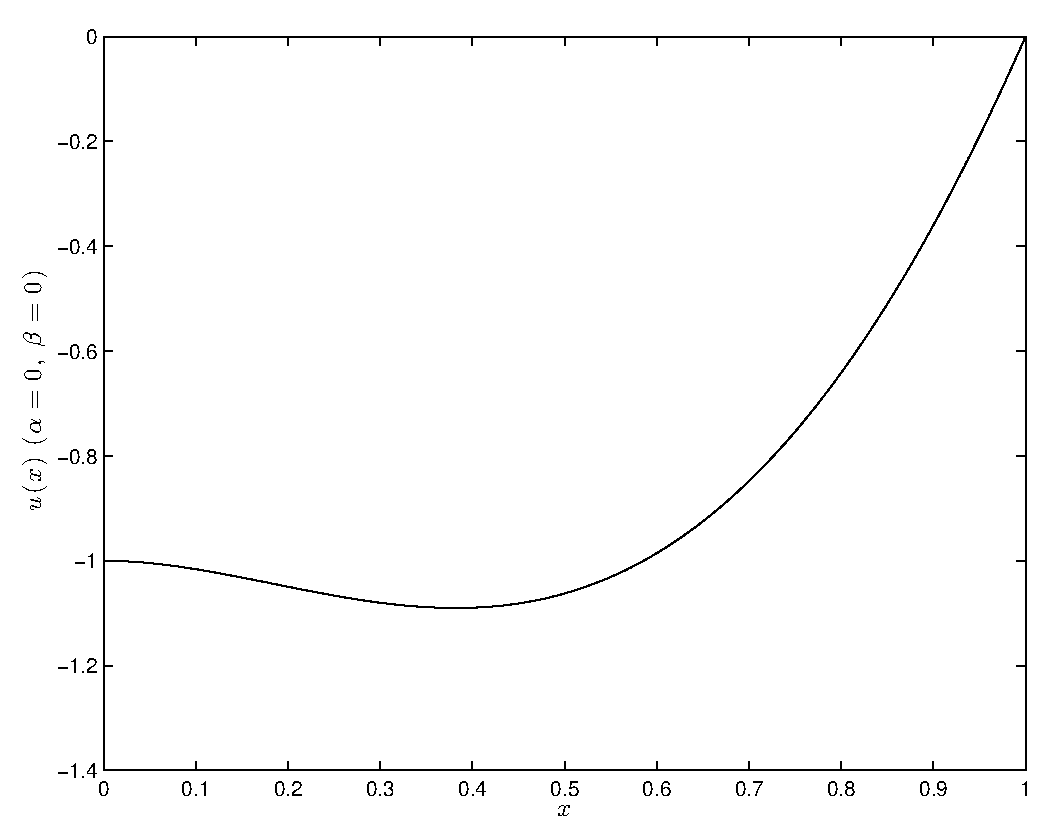
\includegraphics[scale=0.7]{hw5b.eps}
\end{center}

\lstinputlisting{HW5b.m}

\vspace*{1em}
\item {[5 points]} The plot and code used to create it are below.

\begin{center}
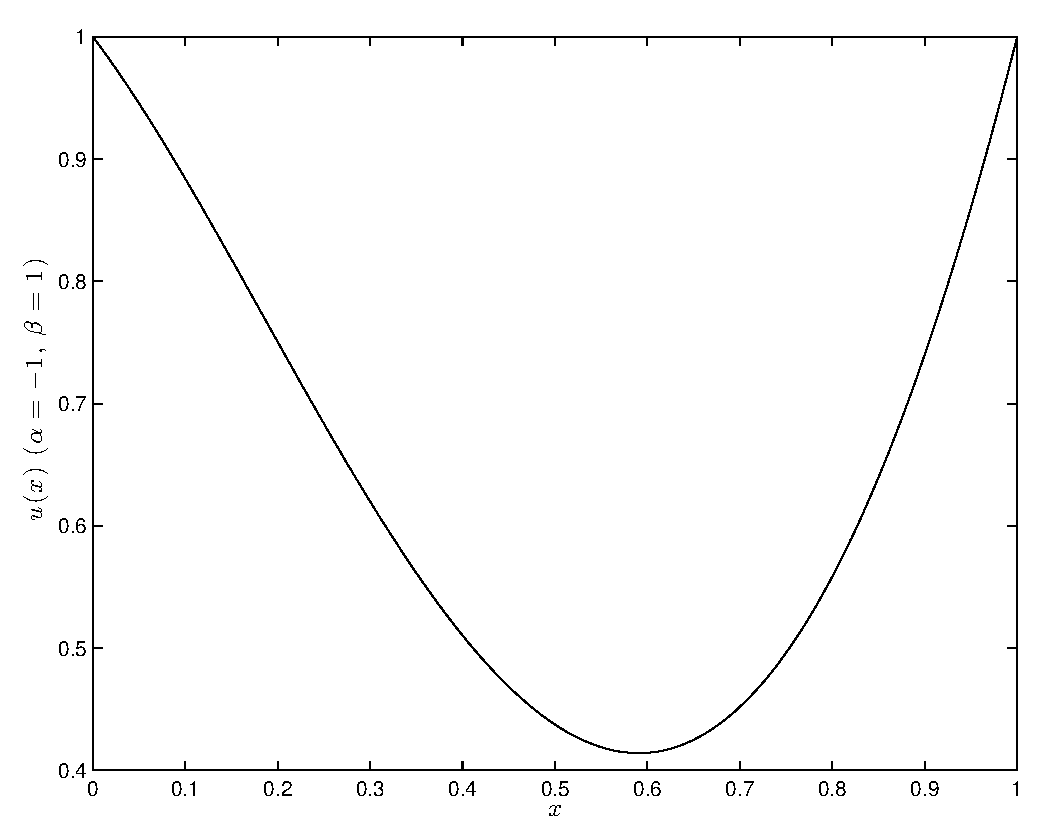
\includegraphics[scale=0.7]{hw5c.eps}
\end{center}

\lstinputlisting{HW5c.m}

\end{enumerate}
\end{solution}